% vim: set spell spelllang=en tw=100 et sw=4 sts=4 :

\documentclass[a0paper]{tikzposter}

\usepackage{complexity}
\usepackage{wrapfig}
\usepackage{microtype}
\usepackage{gnuplot-lua-tikz}
\usepackage{amssymb}
\usepackage{amsmath}
\usepackage{sfmath}

\usepackage{lmodern}
\renewcommand*\familydefault{\sfdefault}
\usepackage[T1]{fontenc}

\title{Heuristics and Really Hard Instances for Subgraph Isomorphism Problems}
\author{Ciaran McCreesh, Patrick Prosser and James Trimble}
\institute{University of Glasgow, Glasgow, Scotland}
\titlegraphic{
\includegraphics[keepaspectratio=true,scale=3.5]{UoG_keyline.pdf}}

\settitle{
    \begin{tikzpicture}
        \node (T) [inner sep=0pt] {\begin{minipage}{\linewidth}
                \color{titlefgcolor}
                {\bfseries \Huge \hspace*{10mm}Heuristics and Really Hard Instances for \\
                \hspace*{10mm}Subgraph Isomorphism Problems \par}
                \vspace*{1em}
                {\Large {\bfseries \hspace{10mm}\@author}, \@institute}
        \end{minipage}};

        \node at (T.east) [anchor=center, inner sep=0pt, xshift=-12cm] {\@titlegraphic};
    \end{tikzpicture}
}

% University of Glasgow standard colours
\definecolor{uofguniversityblue}{rgb}{0, 0.219608, 0.396078}

\definecolor{uofgheather}{rgb}{0.356863, 0.32549, 0.490196}
\definecolor{uofgaquamarine}{rgb}{0.603922, 0.72549, 0.678431}
\definecolor{uofgslate}{rgb}{0.309804, 0.34902, 0.380392}
\definecolor{uofgrose}{rgb}{0.823529, 0.470588, 0.709804}
\definecolor{uofgmocha}{rgb}{0.709804, 0.564706, 0.47451}

\definecolor{uofglawn}{rgb}{0.517647, 0.741176, 0}
\definecolor{uofgcobalt}{rgb}{0, 0.615686, 0.92549}
\definecolor{uofgturquoise}{rgb}{0, 0.709804, 0.819608}
\definecolor{uofgsunshine}{rgb}{1.0, 0.862745, 0.211765}
\definecolor{uofgpumpkin}{rgb}{1.0, 0.72549, 0.282353}
\definecolor{uofgthistle}{rgb}{0.584314, 0.070588, 0.447059}
\definecolor{uofgpillarbox}{rgb}{0.701961, 0.047059, 0}
\definecolor{uofglavendar}{rgb}{0.356863, 0.301961, 0.580392}

\definecolor{uofgsandstone}{rgb}{0.321569, 0.278431, 0.231373}
\definecolor{uofgforest}{rgb}{0, 0.317647, 0.2}
\definecolor{uofgburgundy}{rgb}{0.490196, 0.133333, 0.223529}
\definecolor{uofgrust}{rgb}{0.603922, 0.227451, 0.023529}

\definecolorstyle{UofG}{
}{
    % Background Colors
    \colorlet{backgroundcolor}{uofgsandstone!80!white}
    \colorlet{framecolor}{black}
    % Title Colors
    \colorlet{titlefgcolor}{white}
    \colorlet{titlebgcolor}{uofguniversityblue}
    % Block Colors
    \colorlet{blocktitlebgcolor}{white}
    \colorlet{blocktitlefgcolor}{uofguniversityblue}
    \colorlet{blockbodybgcolor}{white}
    \colorlet{blockbodyfgcolor}{black}
    % Innerblock Colors
    \colorlet{innerblocktitlebgcolor}{uofguniversityblue}
    \colorlet{innerblocktitlefgcolor}{black}
    \colorlet{innerblockbodybgcolor}{uofgsandstone}
    \colorlet{innerblockbodyfgcolor}{black}
    % Note colors
    \colorlet{notefgcolor}{black}
    \colorlet{notebgcolor}{uofgrust}
    \colorlet{noteframecolor}{red}
}

\usetheme{Autumn}
\usecolorstyle{UofG}

\tikzposterlatexaffectionproofoff

\useblockstyle[bodyverticalshift=-1cm, roundedcorners=1]{Default}

\renewcommand{\Huge}{\fontsize{77.2}{96}\selectfont}

% Styles for drawings

\tikzset{edge/.style={line width=3pt, color=uofgsandstone}}
\tikzset{ledge/.style={line width=3pt, color=uofgsandstone!40!white}}
\tikzset{hedge/.style={line width=3pt, color=uofgsandstone, dashed}}

\setlength\intextsep{0pt}

\begin{document}
\maketitle

{
    \colorlet{blockbodybgcolor}{uofgcobalt}
    \colorlet{blocktitlebgcolor}{uofgcobalt}
    \block[bodyverticalshift=0cm, bodyinnersep=3mm]{}{
        \centering\begin{minipage}{0.94\textwidth}
            We show how to generate \textbf{really hard} random instances for \textbf{subgraph
            isomorphism} problems. For the non-induced variant, we predict and observe a phase
            transition between satisfiable and unsatisfiable instances, with a corresponding
            complexity peak seen in \textbf{three different solvers}. For the induced variant, much
            richer behaviour is observed, and \textbf{constrainedness} gives a better measure of
            difficulty than does proximity to a phase transition. We also discuss \textbf{variable
            and value ordering} heuristics, and their relationship to the \textbf{expected number of
            solutions}.
        \end{minipage}
    }
}

\begin{columns}
\column{0.5}

\block{Subgraph Isomorphism (Finding Patterns in Graphs)}{
\begin{wrapfigure}[11]{r}{0.46\linewidth}
    \begin{center}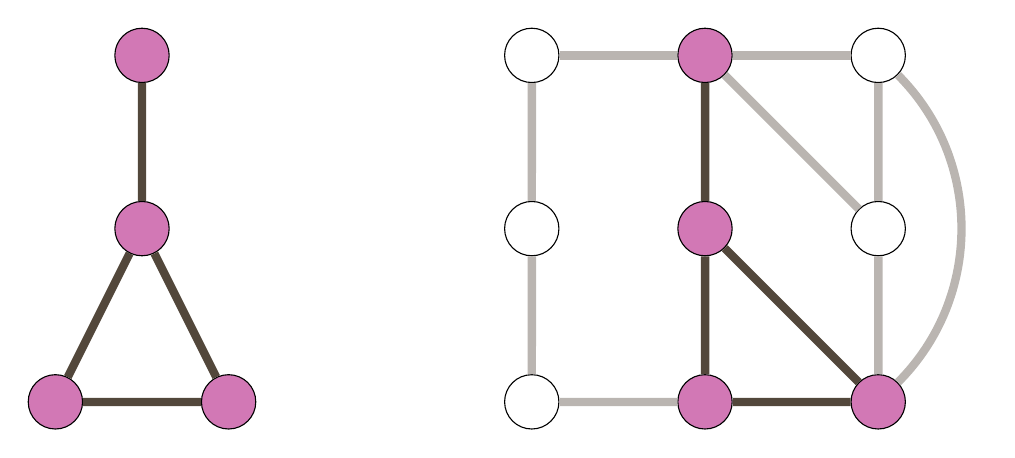
\begin{tikzpicture}[scale=1.1]%{{{
        \node[draw, circle, fill=uofgrose, inner sep=5pt, font=\bfseries] (Na) at (1,  0)
        {\vphantom{0}};
        \node[draw, circle, fill=uofgrose, inner sep=5pt, font=\bfseries] (Nb) at (1, -2)
        {\vphantom{0}};
        \node[draw, circle, fill=uofgrose, inner sep=5pt, font=\bfseries] (Nc) at (0, -4)
        {\vphantom{0}};
        \node[draw, circle, fill=uofgrose, inner sep=5pt, font=\bfseries] (Nd) at (2, -4)
        {\vphantom{0}};

        \draw [edge] (Na) -- (Nb);
        \draw [edge] (Nb) -- (Nc);
        \draw [edge] (Nc) -- (Nd);
        \draw [edge] (Nb) -- (Nd);

        \node[draw, circle, fill=uofgrose, inner sep=5pt, font=\bfseries] (N1) at (7.5,  0) {\vphantom{0}};
        \node[draw, circle, fill=white, inner sep=5pt, font=\bfseries] (N2) at (9.5,  0) {\vphantom{0}};
        \node[draw, circle, fill=uofgrose, inner sep=5pt, font=\bfseries] (N3) at (7.5, -2) {\vphantom{0}};
        \node[draw, circle, fill=white, inner sep=5pt, font=\bfseries] (N4) at (9.5, -2) {\vphantom{0}};
        \node[draw, circle, fill=uofgrose, inner sep=5pt, font=\bfseries] (N5) at (7.5, -4) {\vphantom{0}};
        \node[draw, circle, fill=uofgrose, inner sep=5pt, font=\bfseries] (N6) at (9.5, -4) {\vphantom{0}};
        \node[draw, circle, fill=white, inner sep=5pt, font=\bfseries] (N7) at (5.5,  0) {\vphantom{0}};
        \node[draw, circle, fill=white, inner sep=5pt, font=\bfseries] (N8) at (5.5, -2) {\vphantom{0}};
        \node[draw, circle, fill=white, inner sep=5pt, font=\bfseries] (N9) at (5.5, -4) {\vphantom{0}};

        \draw [ledge] (N1) -- (N2);
        \draw [edge] (N1) -- (N3);
        \draw [ledge] (N1) -- (N4);
        \draw [ledge] (N2) -- (N4);
        \draw [edge] (N3) -- (N5);
        \draw [edge] (N3) -- (N6);
        \draw [ledge] (N4) -- (N6);
        \draw [edge] (N5) -- (N6);
        \draw [ledge] (N2) to [in=45, out=315] (N6);
        \draw [ledge] (N1) -- (N7);
        \draw [ledge] (N5) -- (N9);
        \draw [ledge] (N7) -- (N8);
        \draw [ledge] (N8) -- (N9);
    \end{tikzpicture}\end{center}

    \vspace*{1.5cm}

    \begin{center}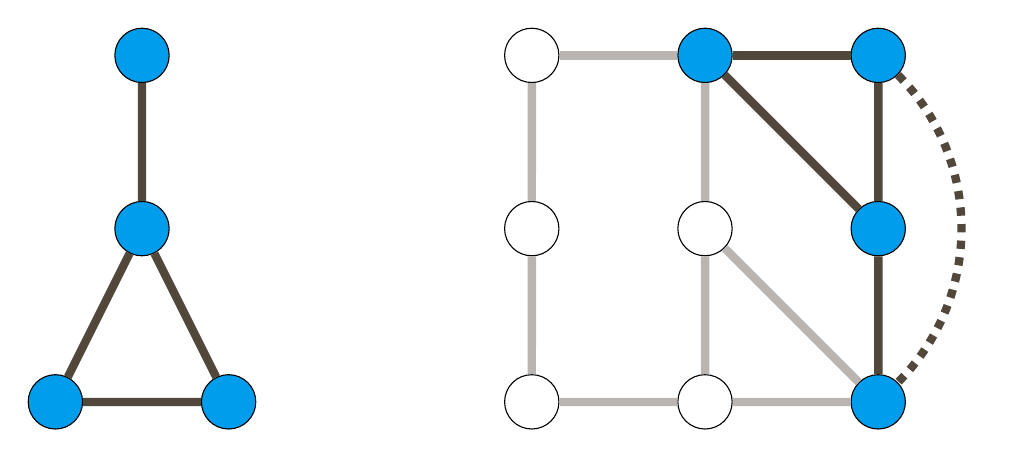
\begin{tikzpicture}[scale=1.1]%{{{
        \node[draw, circle, fill=uofgcobalt, inner sep=5pt, font=\bfseries] (Na) at (1,  0)
        {\vphantom{0}};
        \node[draw, circle, fill=uofgcobalt, inner sep=5pt, font=\bfseries] (Nb) at (1, -2)
        {\vphantom{0}};
        \node[draw, circle, fill=uofgcobalt, inner sep=5pt, font=\bfseries] (Nc) at (0, -4)
        {\vphantom{0}};
        \node[draw, circle, fill=uofgcobalt, inner sep=5pt, font=\bfseries] (Nd) at (2, -4)
        {\vphantom{0}};

        \draw [edge] (Na) -- (Nb);
        \draw [edge] (Nb) -- (Nc);
        \draw [edge] (Nc) -- (Nd);
        \draw [edge] (Nb) -- (Nd);

        \node[draw, circle, fill=uofgcobalt, inner sep=5pt, font=\bfseries] (N1) at (7.5,  0) {\vphantom{0}};
        \node[draw, circle, fill=uofgcobalt, inner sep=5pt, font=\bfseries] (N2) at (9.5,  0) {\vphantom{0}};
        \node[draw, circle, fill=white, inner sep=5pt, font=\bfseries] (N3) at (7.5, -2) {\vphantom{0}};
        \node[draw, circle, fill=uofgcobalt, inner sep=5pt, font=\bfseries] (N4) at (9.5, -2) {\vphantom{0}};
        \node[draw, circle, fill=white, inner sep=5pt, font=\bfseries] (N5) at (7.5, -4) {\vphantom{0}};
        \node[draw, circle, fill=uofgcobalt, inner sep=5pt, font=\bfseries] (N6) at (9.5, -4) {\vphantom{0}};
        \node[draw, circle, fill=white, inner sep=5pt, font=\bfseries] (N7) at (5.5,  0) {\vphantom{0}};
        \node[draw, circle, fill=white, inner sep=5pt, font=\bfseries] (N8) at (5.5, -2) {\vphantom{0}};
        \node[draw, circle, fill=white, inner sep=5pt, font=\bfseries] (N9) at (5.5, -4) {\vphantom{0}};

        \draw [edge] (N1) -- (N2);
        \draw [ledge] (N1) -- (N3);
        \draw [edge] (N1) -- (N4);
        \draw [edge] (N2) -- (N4);
        \draw [ledge] (N3) -- (N5);
        \draw [ledge] (N3) -- (N6);
        \draw [edge] (N4) -- (N6);
        \draw [ledge] (N5) -- (N6);
        \draw [hedge] (N2) to [in=45, out=315] (N6);
        \draw [ledge] (N1) -- (N7);
        \draw [ledge] (N5) -- (N9);
        \draw [ledge] (N7) -- (N8);
        \draw [ledge] (N8) -- (N9);
    \end{tikzpicture}\end{center}
\end{wrapfigure}

The \textbf{non-induced subgraph isomorphism problem} is to find an injective mapping from a given
pattern graph to a given target graph which preserves adjacency---in essence, we are ``finding a
copy of'' the pattern inside the target.

\bigskip

The \textbf{induced} variant of the problem additionally requires that the mapping preserve
non-adjacency, so there are no ``extra edges'' in the copy of the pattern that we find. The top
example is induced, whereas the bottom example is not, due to the dashed edge.

\bigskip

Despite these problems being \NP-complete, modern practical subgraph isomorphism algorithms can
handle problem instances with many hundreds of vertices in the pattern graph, and up to \textbf{ten thousand
vertices} in the target graph, leading to successful application in areas such as \textbf{computer
vision}, \textbf{biochemistry}, and \textbf{pattern recognition}. However, these algorithms cannot
handle arbitrary instances of this size---here we generate instances with thirty and one hundred and
fifty vertices respectively which cannot be solved within one hour.
}

\block{The Expected Number of Solutions, and Heuristics}{

If we randomly generate a pattern graph with $p$ vertices and density $d_p$, and a target graph
with $t$ vertices and density $d_t$, the \textbf{expected number of solutions} to the non-induced
isomorphism problem is \[
    \mathsf{\langle Sol \rangle = t \cdot (t - 1) \cdot \ldots \cdot (t - p + 1)\cdot {d_t}^{d_p \cdot
    \binom{p}{2}} } \textnormal{.} \]

\bigskip

By considering when $\mathsf{\langle Sol \rangle = 1}$, we can \textbf{estimate the location} of the
satisfiable / unsatisfiable phase transition. (This is not entirely accurate due to variance,
particularly when the pattern is very sparse or very dense).

\bigskip

We can also use this formula to recover \textbf{variable} and \textbf{value ordering heuristics}: we
should make branching decisions which maximise the expected number of solutions during search. This
tells us to prefer small domains and pattern vertices of high degree, but target vertices of low
degree, which matches the empirically-determined heuristics used in state of the art solvers.

}

\column{0.5}

\block{Non-Induced Phase Transitions}{
    If we generate random patterns and targets independently, fixing a pattern order of 20 vertices,
    a target order of 150 vertices, a target density of 0.4, and varying the pattern density, the
    familiar phase transition and (solver-independent) complexity peak occurs.

    \vspace*{1em}

    \begin{center}
        \small
        \input{gen-graph-phase-transition}
    \end{center}

    We can also look at what happens if we vary both the pattern and the target density, for
    different orders of pattern. The top row shows satisfiability---the black lines show where
    $\mathsf{\langle Sol \rangle = 1}$. The bottom row shows the search cost for one of the three
    algorithms we consider in the paper. As expected, the ``really hard'' instances are near the
    phase transition.

    \vspace*{0.9em}

    \begin{center}
        \small
        \input{gen-graph-non-induced}
    \end{center}
}

\end{columns}

\block{Induced Phase Transitions}{
\begin{wrapfigure}[24]{r}{0.64\linewidth}\begin{center}
    \small\input{gen-graph-induced}
\end{center}\end{wrapfigure}

    For induced isomorphisms, the behaviour is much richer. We can derive an expected number of
    solutions of \[
        \mathsf{\langle Sol \rangle = t \cdot (t - 1) \cdot \ldots \cdot (t - p + 1)\cdot
                    {d_t}^{d_p \cdot \binom{p}{2}} \cdot {(1 - d_{t})}^{(1 - d_{p}) \cdot \binom{p}{2}} } \textnormal{.} \]

    \bigskip

    Again this predicts a sharp phase transition. When the pattern is small, we see hard instances
    near the phase transition, and easy instances elsewhere. However, when the pattern is larger,
    the central unsatisfiable region \textbf{remains very hard}, even though it is no longer near a
    phase transition.

    \bigskip

    This is not just a weakness of current subgraph isomorphism algorithms: the region is also hard
    for pseudo-boolean and boolean satisfiability solvers, and under reduction to the clique
    problem.

    \bigskip

    The central hard region \emph{is} predicted correctly by \textbf{constrainedness}, as we
    show in the third row of plots. Although far from a phase transition, this region is only
    slightly overconstrained.

    \bigskip

    Looking to maximise $\mathsf{\langle Sol \rangle}$ derives existing variable and value ordering
    heuristics, in the case that both the pattern and target graphs are sparse. The formula suggests
    that algorithms should swap heuristics when the pattern and target are dense---empirically, this
    does indeed give an improvement. However, maximising the expected number of solutions is
    \textbf{not enough to select the best heuristic} in two eighths of the search space (and
    constrainedness does not help).
}

\begin{columns}
\column{0.5}

\block{See the Paper For\ldots}{
    \begin{itemize}
        \item ~ Results from two other subgraph isomorphism algorithms.
        \item ~ Behaviour under reduction to clique, pseudo-boolean, and boolean satisfiability.
        \item ~ Should we alter heuristics based upon the expected number of solutions?
    \end{itemize}
}

\column{0.5}

\block{Future Work}{
    \begin{itemize}
        \item ~ Variance for more accurate predictions (if you can help, please get in touch).
        \item ~ Other random models (degree-bounded, scale-free, \ldots).
        \item ~ Labelled graphs.
    \end{itemize}
}

\end{columns}

{
    \colorlet{blockbodybgcolor}{uofgsandstone!80!white}
    \colorlet{blocktitlebgcolor}{uofgsandstone!80!white}
    \block[bodyverticalshift=-0.5cm]{}{
        This work was supported by the Engineering and Physical Sciences Research Council [grant
        number EP/K503058/1]. \hfill \texttt{c.mccreesh.1@research.gla.ac.uk}
    }
}

\end{document}

